\documentclass[tikz,border=10pt]{standalone}
% Shared look for every TikZ diagram. Load with \input{../../tools/tikz-style.tex}
\usepackage[T1]{fontenc}
\usepackage{lmodern}
\renewcommand{\sfdefault}{lmr}  % diagrams use the same serif as the text
\usetikzlibrary{arrows.meta, positioning, shapes.geometric, calc, fit, backgrounds}
\definecolor{cblue}{HTML}{4C78A8}
\definecolor{corange}{HTML}{F58518}
\definecolor{cgreen}{HTML}{54A24B}
\definecolor{cred}{HTML}{E45756}
\definecolor{cpurple}{HTML}{B279A2}
\definecolor{cgrey}{HTML}{6B6B6B}
\tikzset{
  every picture/.style={font=\sffamily, line width=1.2pt},
  box/.style={draw=#1, fill=#1!12, rounded corners=4pt, align=center, inner sep=7pt, minimum height=1.1cm},
  box/.default=cgrey,
  arrow/.style={-{Stealth[length=3mm]}, draw=cgrey, line width=1.4pt},
  title/.style={font=\sffamily\bfseries\Large},
  note/.style={font=\sffamily\small, text=cgrey, align=center},
}
\AtBeginDocument{\hyphenpenalty=10000 \exhyphenpenalty=10000}

\begin{document}
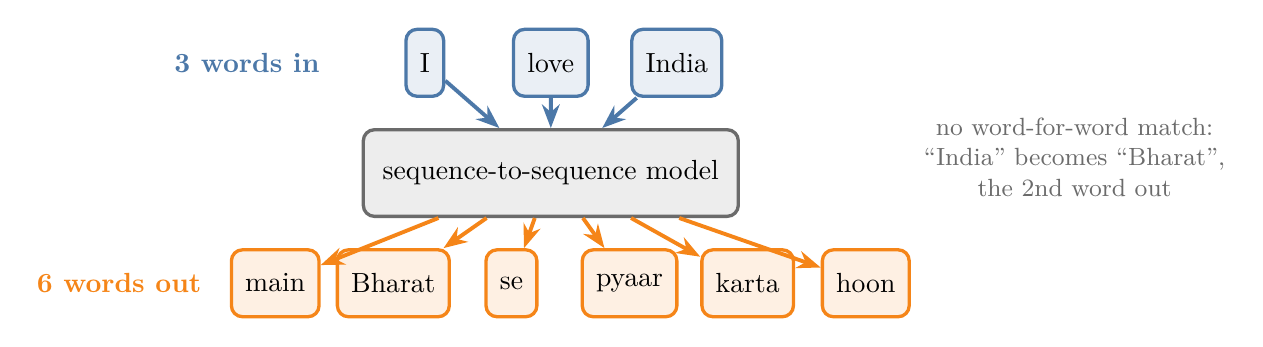
\begin{tikzpicture}[i/.style={box=cblue, inner sep=5pt, minimum height=0.85cm, font=\sffamily},
  o/.style={box=corange, inner sep=5pt, minimum height=0.85cm, font=\sffamily}]
  \foreach \w [count=\k] in {I, love, India} \node[i] (i\k) at (1.6*\k+1.2,1.8) {\w};
  \foreach \w [count=\k] in {main, Bharat, se, pyaar, karta, hoon} \node[o] (o\k) at (1.5*\k-0.6,-1.0) {\w};
  \node[anchor=east, font=\sffamily\bfseries, text=cblue] at (1.6,1.8) {3 words in};
  \node[anchor=east, font=\sffamily\bfseries, text=corange] at (0.1,-1.0) {6 words out};
  \node[box=cgrey, minimum width=4.0cm] (m) at (4.4,0.4) {sequence-to-sequence model};
  \foreach \k in {1,2,3} \draw[arrow, draw=cblue] (i\k) -- (m);
  \foreach \k in {1,...,6} \draw[arrow, draw=corange] (m) -- (o\k);
  \node[note, anchor=west] at (9.0,0.6) {no word-for-word match:\\``India'' becomes ``Bharat'',\\the 2nd word out};
\end{tikzpicture}
\end{document}
